\section{Base de données}
\label{sec:BD}


\subsection{Création de la base de données}
\label{subsec:creation-db}

La base de données est composée de huit tables contenant toutes les données utiles au bon fonctionnement du site. \\

Les six tables de la figure~\ref{fig:db2} ont été créées en plus de celles ajoutées par Laravel\footnote{La table \textbf{users} a été créée par Laravel, mais modifiée afin de répondre aux besoins du site.}. \\
Il y a la table :
\begin{itemize}
    
    \item \textbf{users} qui contient tout ce qui concerne les utilisateurs;
    
    \item \textbf{comments} qui contient la liste des commentaires;
    
    \item \textbf{courses} qui contient les informations des cours;
    
    \item \textbf{chapters} qui contient les chapitres;
    
    \item \textbf{enrollments} qui contient la liste des inscriptions aux cours;
    
    \item \textbf{tests} qui contient les tests.
    
\end{itemize} 

\vspace{0.5cm}

\begin{figure}[h]
  \centering
  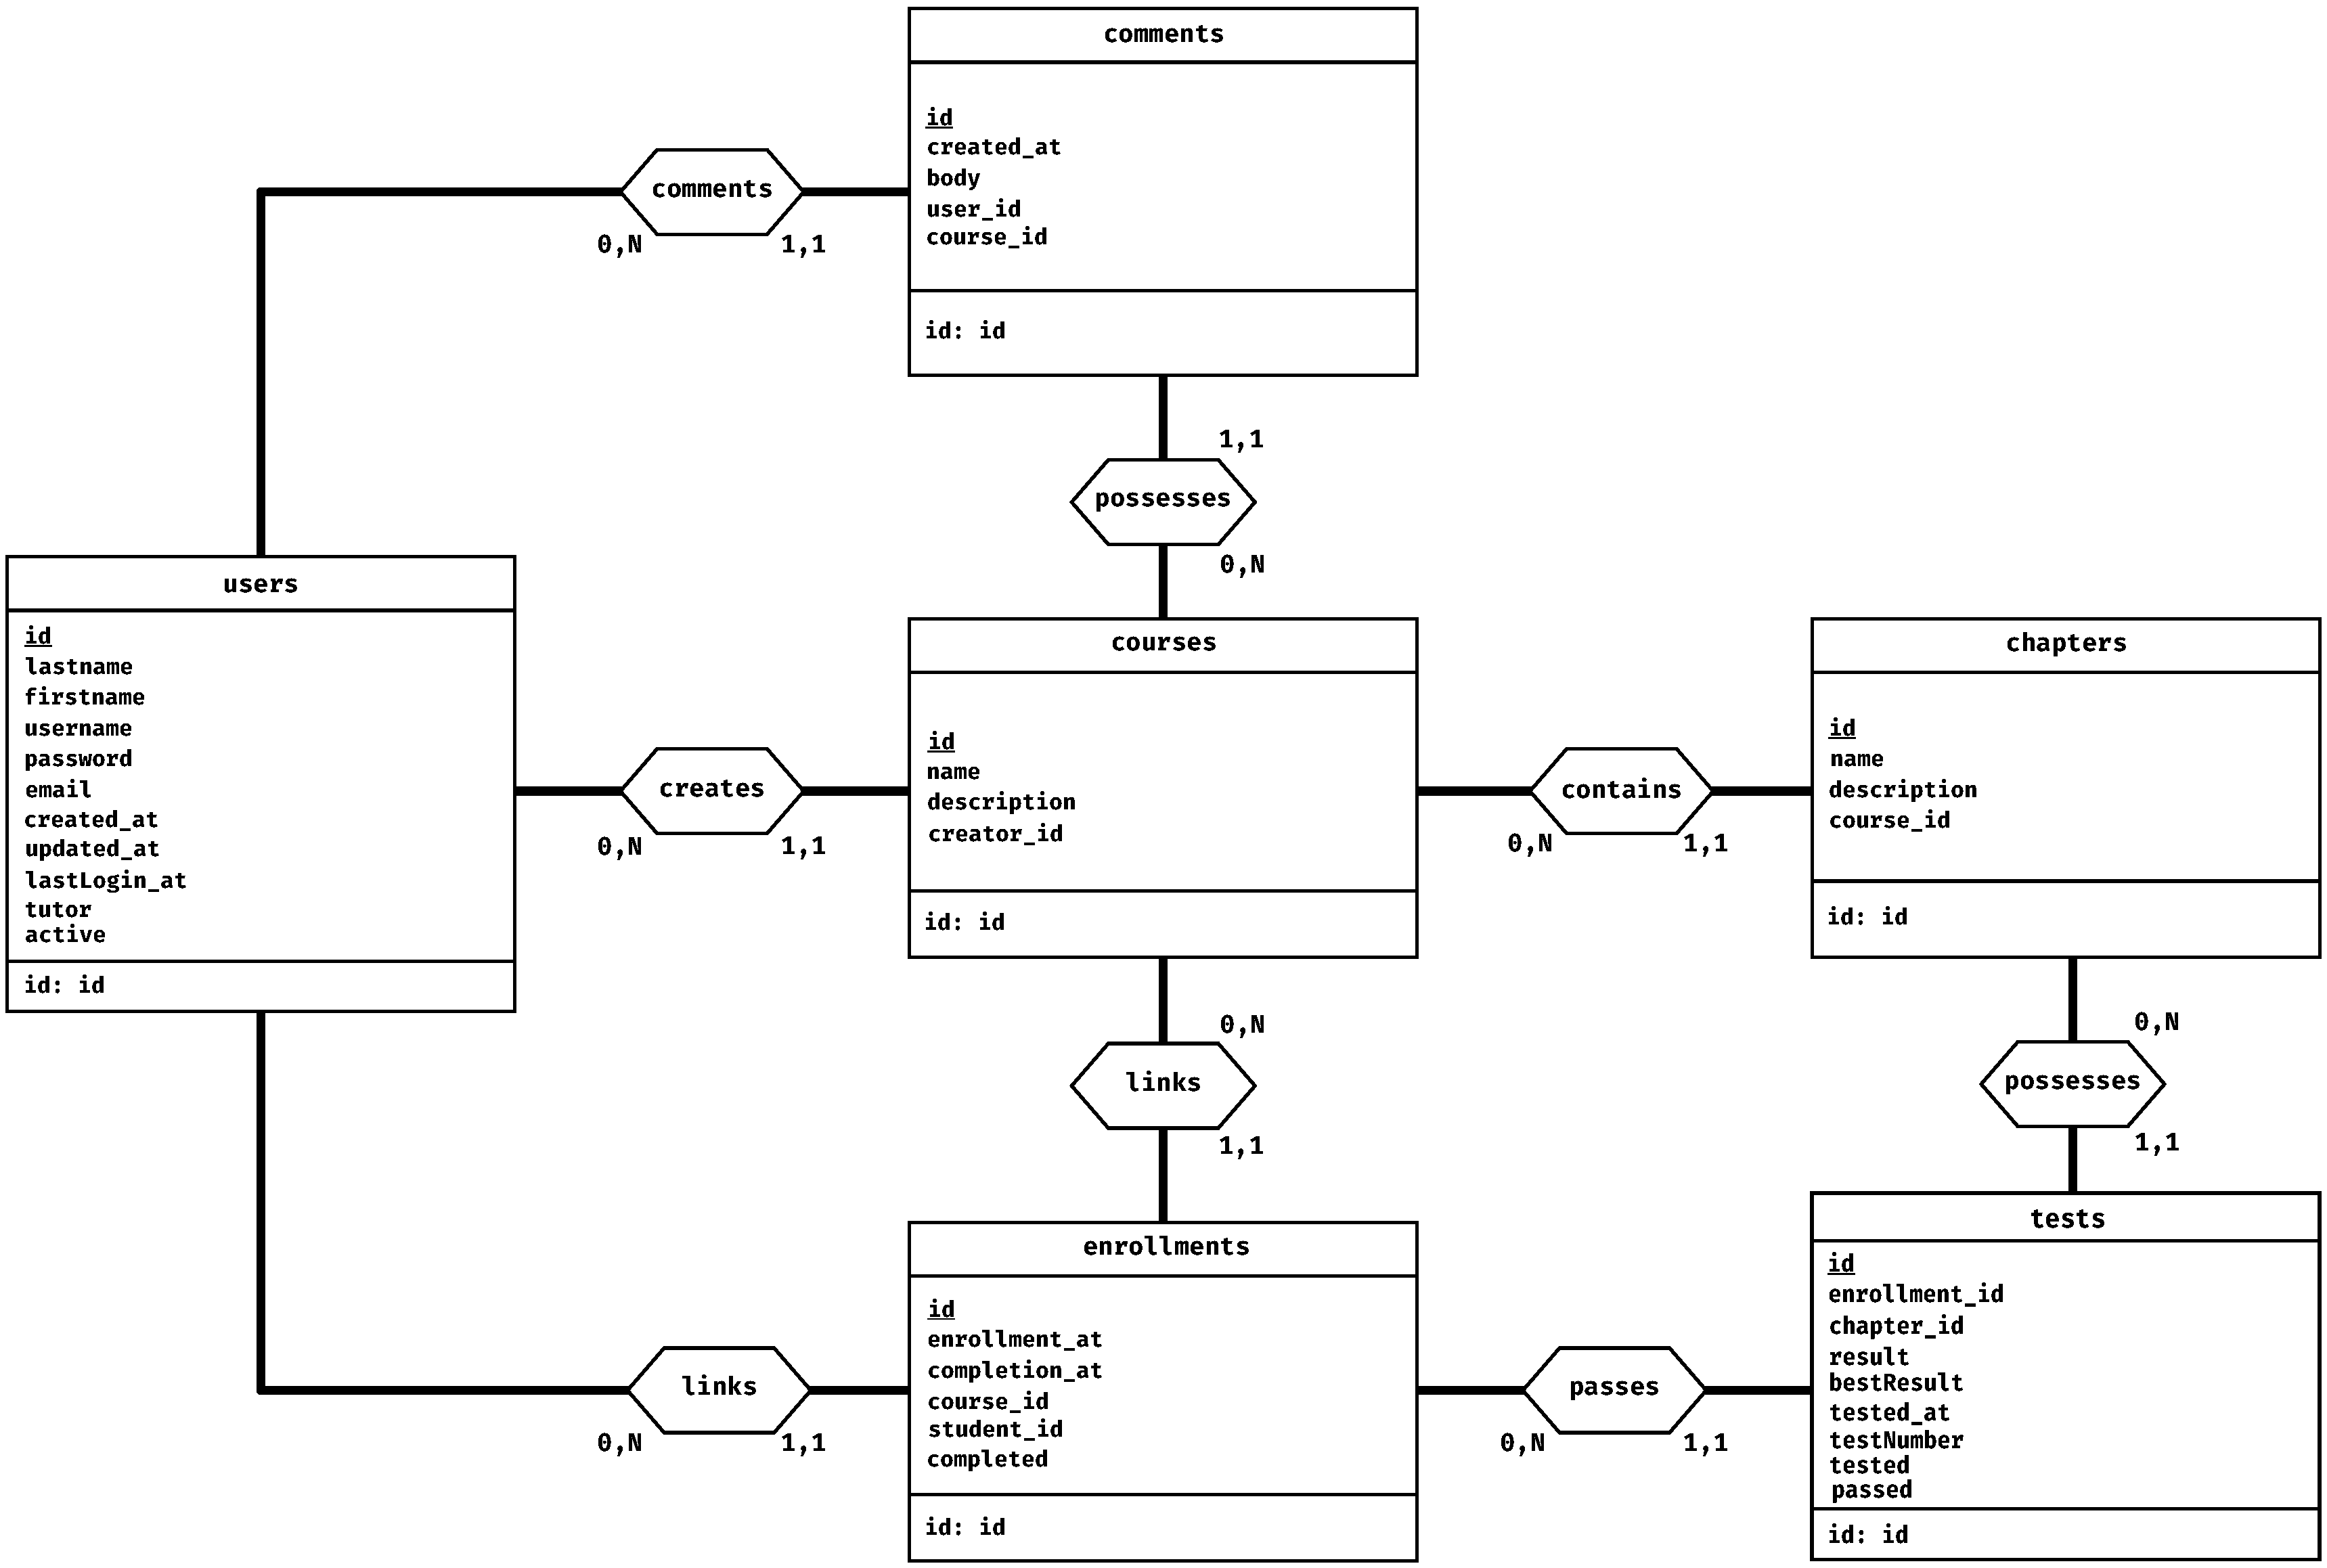
\includegraphics[width=\textwidth]
  {textures/images/DB/Student-Tutor.pdf}
  %\caption[Figure 1]{Schéma conceptuel de la base de données}
  \caption{Schéma conceptuel de la base de données}
  \label{fig:db2}
\end{figure}

\newpage

Le framework Laravel a donc créé trois tables dont \textbf{users}.\\
Les deux autres tables sont \textbf{migrations} et \textbf{password\_resets}.\\
La première gère les migrations \textit{(par exemple : la création des différentes tables)}. \\
La seconde gère la réinitialisation des mots de passe.

\vspace{0.5cm}

\begin{figure}[h]
  \centering
  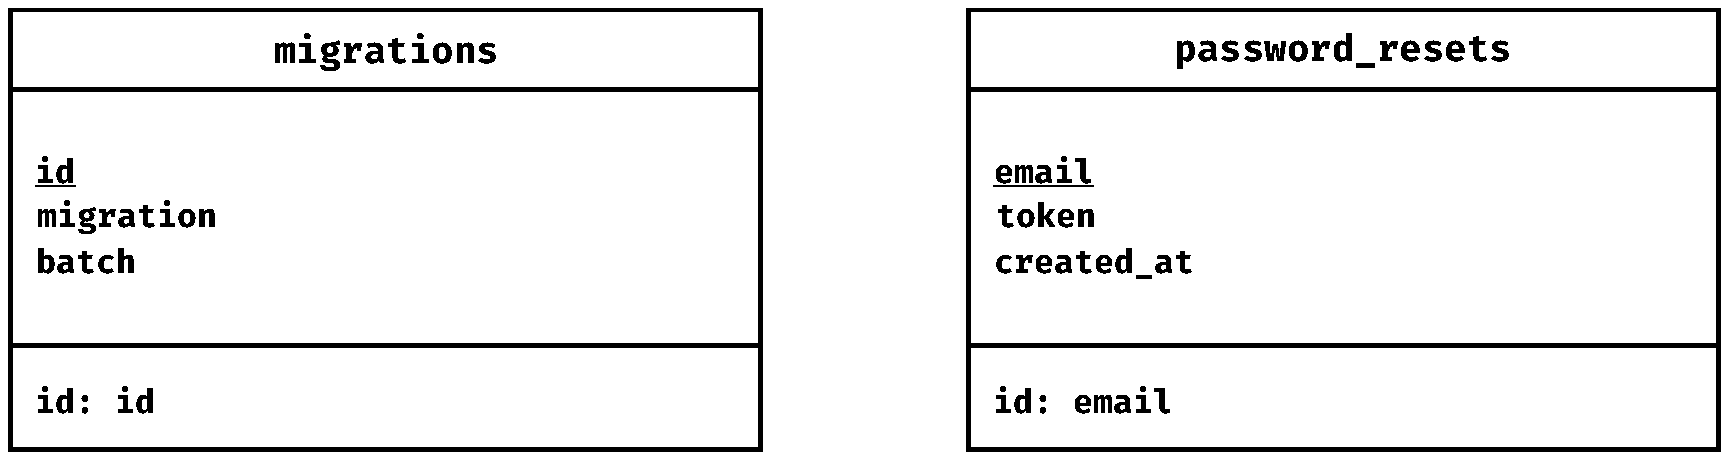
\includegraphics[width=\textwidth]
  {textures/images/DB/Other-Laravel.pdf}
  \caption{Tables créées par Laravel}
  \label{fig:db1}
\end{figure}

\vspace{0.5cm}


\newpage


\subsection{Vue détaillée}
\label{sec:vue-details}
Dans cette section, chaque table sera décrite ainsi que son fonctionnement.


\subsubsection{Table \textit{users}}
\label{sec:table-users}
C'est la table contenant les données de chaque utilisateur et l'état de leur compte.\\
Un utilisateur peut s'inscrire à des cours ou écrire des commentaires et des cours.

Les différents champs sont :

\begin{itemize}
    
    \item[$\bullet$] \textbf{id} est l'identifiant unique de l'utilisateur.\\
    Il sert de clé primaire à la table et est auto-incrémenté à partir de un.
    
    \item[$\bullet$] \textbf{lastname} est le nom de famille de l'utilisateur.
    
    \item[$\bullet$] \textbf{firstname} est le prénom de l'utilisateur.
    
    \item[$\bullet$] \textbf{username} est le nom d'utilisateur unique choisi lors de l'inscription.
    
    \item[$\bullet$] \textbf{password} est le mot de passe de l'utilisateur. Il a une taille minimale de 6 caractères, pouvant être composé de caractères alphanumériques, de tirets et de tirets bas \textit{(underscore)}.\\
    Celui-ci est haché \footnote{\href{https://fr.wikipedia.org/wiki/Fonction\_de\_hachage\_cryptographique}{Wikipédia, Fonction de hachage cryptographique :  https://fr.wikipedia.org/wiki/Hachage}} à l'aide de \textit{Bcrypt} qui est une fonction de hachage incluse dans Laravel.
    
    \item[$\bullet$] \textbf{email} contient l'adresse mail de l'utilisateur.\\
    Ce champ est unique, vu qu'il sert à la connexion de l'utilisateur.
    
    \item[$\bullet$] \textbf{created\_at} contient la date et l'heure de création de l'utilisateur.
    
    \item[$\bullet$] \textbf{updated\_at} contient la date et l'heure de modification de l'utilisateur.
    
    \item[$\bullet$] \textbf{lastLogin\_at} contient la date et l'heure de la dernière connexion de l'utilisateur.
    
    \item[$\bullet$] \textbf{tutor} indique si l'utilisateur a déjà un ou plusieurs cours \textit{(valeur à 1)}, sinon ce sera la valeur par défaut \textit{(valeur à 0)}.
    
    \item[$\bullet$] \textbf{active} donne l'état du compte de l'utilisateur:
    
    \begin{itemize}
        
        \item \textbf{0} indique que le compte est inactif.\\
        Cela signifie que le compte a été supprimé ou que l'administrateur a banni l'utilisateur.
        
        \item \textbf{1} indique que le compte est actif \textit{(par défaut)}.
        
    \end{itemize}
    
\end{itemize}


\newpage


\subsubsection{Table \textit{comments}}
\label{sec:table-comments}
C'est la table contenant les différents commentaires.\\
Ceux-ci sont liés à un utilisateur et à un cours.

Les différents champs sont :

\begin{itemize}
    
    \item[$\bullet$] \textbf{id} est l'identifiant unique du commentaire.\\
    Il sert de clé primaire à la table et est auto-incrémenté à partir de un.
    
    \item[$\bullet$] \textbf{created\_at} contient la date et l'heure de création du commentaire.
    
    \item[$\bullet$] \textbf{body} contient le corps du commentaire.
    
    \item[$\bullet$] \textbf{user\_id} est l'identifiant de l'utilisateur qui l'a écrit.
    
    \item[$\bullet$] \textbf{course\_id} indique le cours auquel le commentaire est lié.
    
\end{itemize}


\subsubsection{Table \textit{courses}}
\label{sec:table-courses}
C'est la table contenant les différents cours.\\
Ceux-ci sont liés à un utilisateur \textit{(son auteur)}, des commentaires et des inscriptions \textit{(enrollments)}.

Les différents champs sont :

\begin{itemize}
    
    \item[$\bullet$] \textbf{id} est l'identifiant unique du cours.\\
    Il sert de clé primaire à la table et est auto-incrémenté à partir de un.
    
    \item[$\bullet$] \textbf{name} est le nom unique du cours.
    
    \item[$\bullet$] \textbf{description} contient la description du cours.
    
    \item[$\bullet$] \textbf{creator\_id} est l'identifiant de l'utilisateur qui l'a écrit.
    
\end{itemize}

\newpage

\subsubsection{Table \textit{chapters}}
\label{sec:table-chapters}
Cette table contient les différents chapitres.\\
Ils sont liés à un cours et à un test.

Les différents champs sont :

\begin{itemize}
    
    \item[$\bullet$] \textbf{id} est l'identifiant unique du chapitre.\\
    Il sert de clé primaire à la table et est auto-incrémenté à partir de un.
    
    \item[$\bullet$] \textbf{name} est le nom du cours.
    
    \item[$\bullet$] \textbf{description} contient la description du chapitre.
    
    \item[$\bullet$] \textbf{course\_id} est l'identifiant du cours auquel il appartient.
    
\end{itemize}


\subsubsection{Table \textit{enrollments}}
\label{sec:table-enrollments}
Cette table contient les différentes inscriptions aux cours.\\
Ils sont liés à un cours, un utilisateur \textit{(celui qui est inscrit)} et à un test.

Les différents champs sont :

\begin{itemize}
    
    \item[$\bullet$] \textbf{id} est l'identifiant unique de l'inscription.\\
    Il sert de clé primaire à la table et est auto-incrémenté à partir de un.
    
    \item[$\bullet$] \textbf{enrollments\_at} contient la date et l'heure d'inscription au cours.
    
    \item[$\bullet$] \textbf{completion\_at} contient la date et l'heure d'achèvement du cours.
    
    \item[$\bullet$] \textbf{course\_id} est l'identifiant du cours auquel l'utilisateur est inscrit.
    
    \item[$\bullet$] \textbf{student\_id} est l'identifiant d'utilisateur inscrit.
    
    \item[$\bullet$] \textbf{completed} donne l'état de l'achèvement du cours :
    
    \begin{itemize}
        
        \item \textbf{0} indique que l'utilisateur n'a pas encore achevé le cours \textit{(par défaut)}.
        
        \item \textbf{1} indique que l'utilisateur a achevé le cours.
        
    \end{itemize}
    
\end{itemize}

\newpage

\subsubsection{Table \textit{tests}}
\label{sec:table-tests}
Cette table contient les différents tests.\\
Ils sont liés à un chapitre et à une inscription.

Les différents champs sont :

\begin{itemize}
    
    \item[$\bullet$] \textbf{id} est l'identifiant unique du test.\\
    Il sert de clé primaire à la table et est auto-incrémenté à partir de un.
    
    \item[$\bullet$] \textbf{enrollment\_id} est le nom du cours.
    
    \item[$\bullet$] \textbf{chapter\_id} est l'identifiant du chapitre auquel il est lié.
    
    \item[$\bullet$] \textbf{result} est le dernier résultat obtenu.
    
    \item[$\bullet$] \textbf{bestResult} est le meilleur résultat obtenu.
    
    \item[$\bullet$] \textbf{tested\_at} contient la date et l'heure du dernier test.
    
    \item[$\bullet$] \textbf{tested} indique si le test a déjà été passé :
    
    \begin{itemize}
        
        \item \textbf{0} l'utilisateur n'a pas encore passé le test \textit{(par défaut)}.
        
        \item \textbf{1} le test a été passé.
        
    \end{itemize}
    
    \item[$\bullet$] \textbf{testNumber} indique combien de fois le test a été passé par l'utilisateur.
    
    \item[$\bullet$] \textbf{passed} indique si le test a déjà été réussi :
    
    \begin{itemize}
        
        \item \textbf{0} l'utilisateur n'a pas encore réussi le test \textit{(par défaut)}.
        
        \item \textbf{1} le test a été réussi.
        
    \end{itemize}
    
\end{itemize}

\newpage

\subsubsection{Table \textit{migrations}}
\label{sec:table-migrations}
Cette table tient un historique des migrations.\\
Les migrations sont utilisées pour créer et définir des bases de données depuis des fichiers \textit{PHP} \textit{(cf. sous-section~\ref{subsec:migration} page~\pageref{subsec:migration})}. 


Les différents champs sont :

\begin{itemize}
    
    \item[$\bullet$] \textbf{id} est l'identifiant unique de la table.\\
    Il sert de clé primaire à la table et est auto-incrémenté à partir de un.
    
    \item[$\bullet$] \textbf{migration} est le nom du fichier \textit{PHP} créant la table.
    
    \item[$\bullet$] \textbf{batch} identifie la migration à laquelle la table a été créée \textit{(1 pour la première)}.
    
\end{itemize}


\subsubsection{Table \textit{password\_resets}}
\label{sec:table-password-resets}
Cette table permet de gérer la réinitialisation des mots de passe en toute sécurité.

Les différents champs sont :

\begin{itemize}
    
    \item[$\bullet$] \textbf{email} est l'identifiant unique de la réinitialisation, l'adresse mail de l'utilisateur qui réinitialise son mot de passe.
    
    \item[$\bullet$] \textbf{token} est le jeton de réinitialisation .
    
    \item[$\bullet$] \textbf{created\_at} contient la date et l'heure de création du jeton de réinitialisation.
    
\end{itemize}

\newpage

\subsection{Sécurité}
\label{subsec:securite}

\subsubsection{Injections SQL}
\label{sec:injections-sql}
Laravel fournit une méthode de protection contre les injections SQL. \\
Celles-ci forment l'une des méthodes d'attaque la plus connue et les plus dangereuses en PHP. \\
Les risques que représente ce genre de faille sont énormes : comme son nom l'indique, cette faille se manifeste lorsqu'il est possible d'injecter ou de modifier une requête SQL. \\
Ceci en injectant des morceaux de code \textit{non filtrés}, généralement par le biais d'un formulaire d'une page du site.

Le constructeur de requête \textit{(Query builder)} de Laravel utilise des instructions préparées de SQL qui rendent les attaques par injection inimaginables. \\
Il n'y a donc pas besoin d'effectuer de traitements sur les données avant de les passer au constructeur de requête. \\
Par contre, les requêtes brutes, utilisées en passant par \textit{DB::raw()}, y sont vulnérables vu que non préparées...

\subsubsection{Attaques CSRF}
\label{sec:attaques-csrf}
Le CSRF, ou Cross Site Request Forgery, est un type de vulnérabilité des services d'authentification web.\\
Le fonctionnement de l'attaque est simple : l'attaquant transmet une requête HTTP falsifiée à un utilisateur authentifié. Celle-ci pointe sur une action interne au site et est exécutée par l'utilisateur authentifié \textit{à son insu} et en utilisant \textit{ses propres droits}.

Une des possibilités de prévention est disponible dans Laravel : l'insertion de jetons de validité dans les formulaires.\\
Un formulaire posté n'est alors accepté que s'il a été produit quelques minutes auparavant : le jeton de validité en sera la preuve. Ce dernier doit être transmis en paramètre et vérifié côté serveur\footnote{\href{https://fr.wikipedia.org/wiki/CSRF}{Wikipédia, Cross-Site Request Forgery :  https://fr.wikipedia.org/wiki/CSRF}}.
